\documentclass[preprint,12pt]{elsarticle}
\usepackage[T1]{fontenc}
\usepackage{lmodern}
\usepackage[utf8]{inputenc}
\usepackage{amsmath,amssymb,amsthm}
\usepackage{booktabs,multirow}
\usepackage{graphicx}
\usepackage{algorithm}
\usepackage{algpseudocode}
\usepackage{tikz}
\usetikzlibrary{arrows.meta,positioning,fit,calc,backgrounds}
\usepackage{hyperref}
\usepackage{xspace}
\newcommand{\ablleaFedAvglocaltra}{0.707}
\newcommand{\ablleaFedAvglocaltraagentic}{0.764}
\newcommand{\ablleaFedAvglocaltraamazon}{0.649}
\newcommand{\ablleaFedAvglocaltracon}{0.866}
\newcommand{\ablleaFedAvglocaltragap}{0.804}
\newcommand{\ablleaFedAvglocaltrairr}{0.741}
\newcommand{\ablleaFedAvglocaltrared}{0.430}
\newcommand{\ablleadensitymatchin}{0.652}
\newcommand{\ablleadensitymatchinagentic}{0.656}
\newcommand{\ablleadensitymatchinamazon}{0.647}
\newcommand{\ablleadensitymatchincon}{0.812}
\newcommand{\ablleadensitymatchingap}{0.775}
\newcommand{\ablleadensitymatchinirr}{0.985}
\newcommand{\ablleadensitymatchinred}{0.102}
\newcommand{\ablleafulllearneddec}{0.742}
\newcommand{\ablleafulllearneddecagentic}{0.832}
\newcommand{\ablleafulllearneddecamazon}{0.652}
\newcommand{\ablleafulllearneddeccon}{0.873}
\newcommand{\ablleafulllearneddecgap}{0.832}
\newcommand{\ablleafulllearneddecirr}{0.800}
\newcommand{\ablleafulllearneddecred}{0.495}
\newcommand{\ablleahyperedgeprior}{0.771}
\newcommand{\ablleahyperedgeprioragentic}{0.806}
\newcommand{\ablleahyperedgeprioramazon}{0.735}
\newcommand{\ablleahyperedgepriorcon}{0.876}
\newcommand{\ablleahyperedgepriorgap}{0.821}
\newcommand{\ablleahyperedgepriorirr}{0.982}
\newcommand{\ablleahyperedgepriorred}{0.466}
\newcommand{\abllealearnedmessage}{0.739}
\newcommand{\abllealearnedmessageagentic}{0.825}
\newcommand{\abllealearnedmessageamazon}{0.652}
\newcommand{\abllealearnedmessagecon}{0.873}
\newcommand{\abllealearnedmessagegap}{0.825}
\newcommand{\abllealearnedmessageirr}{0.800}
\newcommand{\abllealearnedmessagered}{0.490}
\newcommand{\ablleancols}{2}
\newcommand{\ablleapseudoanomalya}{0.584}
\newcommand{\ablleapseudoanomalyaagentic}{0.665}
\newcommand{\ablleapseudoanomalyaamazon}{0.502}
\newcommand{\ablleapseudoanomalyacon}{0.874}
\newcommand{\ablleapseudoanomalyagap}{0.833}
\newcommand{\ablleapseudoanomalyairr}{0.600}
\newcommand{\ablleapseudoanomalyared}{0.025}
\newcommand{\ablstrconjunctivepoo}{0.591}
\newcommand{\ablstrconjunctivepooagentic}{0.639}
\newcommand{\ablstrconjunctivepooamazon}{0.539}
\newcommand{\ablstrconjunctivepoocon}{0.491}
\newcommand{\ablstrconjunctivepoogap}{0.667}
\newcommand{\ablstrconjunctivepooirr}{1.000}
\newcommand{\ablstrconjunctivepoored}{0.321}
\newcommand{\ablstrconjunctivepooxustoller}{0.595}
\newcommand{\ablstrfull}{0.829}
\newcommand{\ablstrfullagentic}{0.865}
\newcommand{\ablstrfullamazon}{0.893}
\newcommand{\ablstrfullcon}{0.893}
\newcommand{\ablstrfullgap}{0.742}
\newcommand{\ablstrfullirr}{1.000}
\newcommand{\ablstrfullred}{0.725}
\newcommand{\ablstrfullxustoller}{0.729}
\newcommand{\ablstrncols}{3}
\newcommand{\ablstrscopepartition}{0.456}
\newcommand{\ablstrscopepartitionagentic}{0.423}
\newcommand{\ablstrscopepartitionamazon}{0.417}
\newcommand{\ablstrscopepartitioncon}{0.636}
\newcommand{\ablstrscopepartitiongap}{0.000}
\newcommand{\ablstrscopepartitionirr}{1.000}
\newcommand{\ablstrscopepartitionred}{0.327}
\newcommand{\ablstrscopepartitionxustoller}{0.528}
\newcommand{\ablstrsignaturesketc}{0.462}
\newcommand{\ablstrsignaturesketcagentic}{0.420}
\newcommand{\ablstrsignaturesketcamazon}{0.437}
\newcommand{\ablstrsignaturesketccon}{0.648}
\newcommand{\ablstrsignaturesketcgap}{0.010}
\newcommand{\ablstrsignaturesketcirr}{1.000}
\newcommand{\ablstrsignaturesketcred}{0.325}
\newcommand{\ablstrsignaturesketcxustoller}{0.528}
\newcommand{\ablstrwildcardvertic}{0.409}
\newcommand{\ablstrwildcardverticagentic}{0.538}
\newcommand{\ablstrwildcardverticamazon}{0.356}
\newcommand{\ablstrwildcardverticcon}{0.089}
\newcommand{\ablstrwildcardverticgap}{0.667}
\newcommand{\ablstrwildcardverticirr}{1.000}
\newcommand{\ablstrwildcardverticred}{0.054}
\newcommand{\ablstrwildcardverticxustoller}{0.334}
\newcommand{\costagenticctx}{14}
\newcommand{\costagenticmodel}{85}
\newcommand{\costamazonctx}{17}
\newcommand{\costamazonmodel}{94}
\newcommand{\costxustollerctx}{24}
\newcommand{\costxustollermodel}{92}
\newcommand{\mainagenticG}{0.249}
\newcommand{\mainagenticGap}{0.514}
\newcommand{\mainagenticGcon}{0.094}
\newcommand{\mainagenticGconprec}{0.356}
\newcommand{\mainagenticGconrec}{0.061}
\newcommand{\mainagenticGgap}{0.700}
\newcommand{\mainagenticGgapprec}{0.539}
\newcommand{\mainagenticGgaprec}{1.000}
\newcommand{\mainagenticGirr}{0.200}
\newcommand{\mainagenticGirrprec}{0.200}
\newcommand{\mainagenticGirrrec}{0.200}
\newcommand{\mainagenticGred}{0.000}
\newcommand{\mainagenticGredprec}{0.000}
\newcommand{\mainagenticGredrec}{0.000}
\newcommand{\mainagenticH}{0.475}
\newcommand{\mainagenticHap}{0.531}
\newcommand{\mainagenticHcon}{0.201}
\newcommand{\mainagenticHconprec}{0.423}
\newcommand{\mainagenticHconrec}{0.146}
\newcommand{\mainagenticHgap}{0.700}
\newcommand{\mainagenticHgapprec}{0.539}
\newcommand{\mainagenticHgaprec}{1.000}
\newcommand{\mainagenticHirr}{1.000}
\newcommand{\mainagenticHirrprec}{1.000}
\newcommand{\mainagenticHirrrec}{1.000}
\newcommand{\mainagenticHred}{0.000}
\newcommand{\mainagenticHredprec}{0.000}
\newcommand{\mainagenticHredrec}{0.000}
\newcommand{\mainagenticL}{0.826}
\newcommand{\mainagenticLap}{0.887}
\newcommand{\mainagenticLcon}{0.811}
\newcommand{\mainagenticLconprec}{0.686}
\newcommand{\mainagenticLconrec}{0.992}
\newcommand{\mainagenticLgap}{0.851}
\newcommand{\mainagenticLgapprec}{0.868}
\newcommand{\mainagenticLgaprec}{0.846}
\newcommand{\mainagenticLirr}{1.000}
\newcommand{\mainagenticLirrprec}{1.000}
\newcommand{\mainagenticLirrrec}{1.000}
\newcommand{\mainagenticLoc}{0.270}
\newcommand{\mainagenticLocap}{0.388}
\newcommand{\mainagenticLoccon}{0.156}
\newcommand{\mainagenticLocconprec}{0.550}
\newcommand{\mainagenticLocconrec}{0.102}
\newcommand{\mainagenticLocgap}{0.700}
\newcommand{\mainagenticLocgapprec}{0.539}
\newcommand{\mainagenticLocgaprec}{1.000}
\newcommand{\mainagenticLocirr}{0.223}
\newcommand{\mainagenticLocirrprec}{0.182}
\newcommand{\mainagenticLocirrrec}{0.300}
\newcommand{\mainagenticLocred}{0.000}
\newcommand{\mainagenticLocredprec}{0.000}
\newcommand{\mainagenticLocredrec}{0.000}
\newcommand{\mainagenticLred}{0.641}
\newcommand{\mainagenticLredprec}{0.846}
\newcommand{\mainagenticLredrec}{0.518}
\newcommand{\mainagenticR}{0.865}
\newcommand{\mainagenticRFc}{0.515}
\newcommand{\mainagenticRFcap}{0.592}
\newcommand{\mainagenticRFccon}{0.274}
\newcommand{\mainagenticRFcconprec}{0.495}
\newcommand{\mainagenticRFcconrec}{0.192}
\newcommand{\mainagenticRFcgap}{0.684}
\newcommand{\mainagenticRFcgapprec}{0.623}
\newcommand{\mainagenticRFcgaprec}{0.764}
\newcommand{\mainagenticRFcirr}{0.976}
\newcommand{\mainagenticRFcirrprec}{0.961}
\newcommand{\mainagenticRFcirrrec}{0.992}
\newcommand{\mainagenticRFcred}{0.123}
\newcommand{\mainagenticRFcredprec}{0.785}
\newcommand{\mainagenticRFcredrec}{0.067}
\newcommand{\mainagenticRap}{0.807}
\newcommand{\mainagenticRcon}{0.808}
\newcommand{\mainagenticRconprec}{0.678}
\newcommand{\mainagenticRconrec}{1.000}
\newcommand{\mainagenticRgap}{0.853}
\newcommand{\mainagenticRgapprec}{1.000}
\newcommand{\mainagenticRgaprec}{0.745}
\newcommand{\mainagenticRirr}{1.000}
\newcommand{\mainagenticRirrprec}{1.000}
\newcommand{\mainagenticRirrrec}{1.000}
\newcommand{\mainagenticRred}{0.800}
\newcommand{\mainagenticRredprec}{0.668}
\newcommand{\mainagenticRredrec}{1.000}
\newcommand{\mainagenticbest}{0.515}
\newcommand{\mainagenticgain}{+0.351}
\newcommand{\mainagenticp}{6.9\times10^{-6}}
\newcommand{\mainagenticpRL}{0.028}
\newcommand{\mainamazonG}{0.345}
\newcommand{\mainamazonGap}{0.581}
\newcommand{\mainamazonGcon}{0.631}
\newcommand{\mainamazonGconprec}{0.484}
\newcommand{\mainamazonGconrec}{0.918}
\newcommand{\mainamazonGgap}{0.658}
\newcommand{\mainamazonGgapprec}{0.492}
\newcommand{\mainamazonGgaprec}{1.000}
\newcommand{\mainamazonGirr}{0.000}
\newcommand{\mainamazonGirrprec}{0.000}
\newcommand{\mainamazonGirrrec}{0.000}
\newcommand{\mainamazonGred}{0.000}
\newcommand{\mainamazonGredprec}{0.000}
\newcommand{\mainamazonGredrec}{0.000}
\newcommand{\mainamazonH}{0.546}
\newcommand{\mainamazonHap}{0.588}
\newcommand{\mainamazonHcon}{0.634}
\newcommand{\mainamazonHconprec}{0.494}
\newcommand{\mainamazonHconrec}{0.896}
\newcommand{\mainamazonHgap}{0.658}
\newcommand{\mainamazonHgapprec}{0.492}
\newcommand{\mainamazonHgaprec}{1.000}
\newcommand{\mainamazonHirr}{1.000}
\newcommand{\mainamazonHirrprec}{1.000}
\newcommand{\mainamazonHirrrec}{1.000}
\newcommand{\mainamazonHred}{0.000}
\newcommand{\mainamazonHredprec}{0.000}
\newcommand{\mainamazonHredrec}{0.000}
\newcommand{\mainamazonL}{0.698}
\newcommand{\mainamazonLap}{0.903}
\newcommand{\mainamazonLcon}{0.933}
\newcommand{\mainamazonLconprec}{0.891}
\newcommand{\mainamazonLconrec}{0.981}
\newcommand{\mainamazonLgap}{0.766}
\newcommand{\mainamazonLgapprec}{0.651}
\newcommand{\mainamazonLgaprec}{0.950}
\newcommand{\mainamazonLirr}{0.750}
\newcommand{\mainamazonLirrprec}{0.750}
\newcommand{\mainamazonLirrrec}{0.750}
\newcommand{\mainamazonLoc}{0.292}
\newcommand{\mainamazonLocap}{0.519}
\newcommand{\mainamazonLoccon}{0.422}
\newcommand{\mainamazonLocconprec}{0.665}
\newcommand{\mainamazonLocconrec}{0.329}
\newcommand{\mainamazonLocgap}{0.658}
\newcommand{\mainamazonLocgapprec}{0.492}
\newcommand{\mainamazonLocgaprec}{1.000}
\newcommand{\mainamazonLocirr}{0.000}
\newcommand{\mainamazonLocirrprec}{0.000}
\newcommand{\mainamazonLocirrrec}{0.000}
\newcommand{\mainamazonLocred}{0.000}
\newcommand{\mainamazonLocredprec}{0.000}
\newcommand{\mainamazonLocredrec}{0.000}
\newcommand{\mainamazonLred}{0.372}
\newcommand{\mainamazonLredprec}{0.656}
\newcommand{\mainamazonLredrec}{0.283}
\newcommand{\mainamazonR}{0.880}
\newcommand{\mainamazonRFc}{0.560}
\newcommand{\mainamazonRFcap}{0.632}
\newcommand{\mainamazonRFccon}{0.582}
\newcommand{\mainamazonRFcconprec}{0.614}
\newcommand{\mainamazonRFcconrec}{0.555}
\newcommand{\mainamazonRFcgap}{0.667}
\newcommand{\mainamazonRFcgapprec}{0.662}
\newcommand{\mainamazonRFcgaprec}{0.679}
\newcommand{\mainamazonRFcirr}{0.988}
\newcommand{\mainamazonRFcirrprec}{0.977}
\newcommand{\mainamazonRFcirrrec}{1.000}
\newcommand{\mainamazonRFcred}{0.114}
\newcommand{\mainamazonRFcredprec}{0.575}
\newcommand{\mainamazonRFcredrec}{0.064}
\newcommand{\mainamazonRap}{0.830}
\newcommand{\mainamazonRcon}{0.939}
\newcommand{\mainamazonRconprec}{0.885}
\newcommand{\mainamazonRconrec}{1.000}
\newcommand{\mainamazonRgap}{0.866}
\newcommand{\mainamazonRgapprec}{1.000}
\newcommand{\mainamazonRgaprec}{0.768}
\newcommand{\mainamazonRirr}{1.000}
\newcommand{\mainamazonRirrprec}{1.000}
\newcommand{\mainamazonRirrrec}{1.000}
\newcommand{\mainamazonRred}{0.727}
\newcommand{\mainamazonRredprec}{0.578}
\newcommand{\mainamazonRredrec}{1.000}
\newcommand{\mainamazonbest}{0.581}
\newcommand{\mainamazongain}{+0.299}
\newcommand{\mainamazonp}{1.8\times10^{-3}}
\newcommand{\mainamazonpRL}{0.029}
\newcommand{\mainxustollerG}{0.535}
\newcommand{\mainxustollerGap}{0.708}
\newcommand{\mainxustollerGcon}{0.853}
\newcommand{\mainxustollerGconprec}{0.752}
\newcommand{\mainxustollerGconrec}{0.986}
\newcommand{\mainxustollerGgap}{0.600}
\newcommand{\mainxustollerGgapprec}{0.429}
\newcommand{\mainxustollerGgaprec}{1.000}
\newcommand{\mainxustollerGirr}{0.201}
\newcommand{\mainxustollerGirrprec}{0.250}
\newcommand{\mainxustollerGirrrec}{0.168}
\newcommand{\mainxustollerGred}{0.389}
\newcommand{\mainxustollerGredprec}{0.537}
\newcommand{\mainxustollerGredrec}{0.327}
\newcommand{\mainxustollerH}{0.707}
\newcommand{\mainxustollerHap}{0.735}
\newcommand{\mainxustollerHcon}{0.855}
\newcommand{\mainxustollerHconprec}{0.759}
\newcommand{\mainxustollerHconrec}{0.981}
\newcommand{\mainxustollerHgap}{0.600}
\newcommand{\mainxustollerHgapprec}{0.429}
\newcommand{\mainxustollerHgaprec}{1.000}
\newcommand{\mainxustollerHirr}{0.894}
\newcommand{\mainxustollerHirrprec}{0.998}
\newcommand{\mainxustollerHirrrec}{0.827}
\newcommand{\mainxustollerHred}{0.520}
\newcommand{\mainxustollerHredprec}{0.649}
\newcommand{\mainxustollerHredrec}{0.440}
\newcommand{\mainxustollerL}{0.644}
\newcommand{\mainxustollerLap}{0.849}
\newcommand{\mainxustollerLcon}{0.929}
\newcommand{\mainxustollerLconprec}{0.879}
\newcommand{\mainxustollerLconrec}{0.986}
\newcommand{\mainxustollerLgap}{0.643}
\newcommand{\mainxustollerLgapprec}{0.715}
\newcommand{\mainxustollerLgaprec}{0.616}
\newcommand{\mainxustollerLirr}{0.249}
\newcommand{\mainxustollerLirrprec}{0.249}
\newcommand{\mainxustollerLirrrec}{0.250}
\newcommand{\mainxustollerLoc}{0.425}
\newcommand{\mainxustollerLocap}{0.564}
\newcommand{\mainxustollerLoccon}{0.811}
\newcommand{\mainxustollerLocconprec}{0.848}
\newcommand{\mainxustollerLocconrec}{0.782}
\newcommand{\mainxustollerLocgap}{0.600}
\newcommand{\mainxustollerLocgapprec}{0.429}
\newcommand{\mainxustollerLocgaprec}{1.000}
\newcommand{\mainxustollerLocirr}{0.037}
\newcommand{\mainxustollerLocirrprec}{0.114}
\newcommand{\mainxustollerLocirrrec}{0.022}
\newcommand{\mainxustollerLocred}{0.164}
\newcommand{\mainxustollerLocredprec}{0.283}
\newcommand{\mainxustollerLocredrec}{0.115}
\newcommand{\mainxustollerLred}{0.652}
\newcommand{\mainxustollerLredprec}{0.554}
\newcommand{\mainxustollerLredrec}{0.812}
\newcommand{\mainxustollerR}{0.737}
\newcommand{\mainxustollerRFc}{0.756}
\newcommand{\mainxustollerRFcap}{0.808}
\newcommand{\mainxustollerRFccon}{0.849}
\newcommand{\mainxustollerRFcconprec}{0.807}
\newcommand{\mainxustollerRFcconrec}{0.895}
\newcommand{\mainxustollerRFcgap}{0.699}
\newcommand{\mainxustollerRFcgapprec}{0.707}
\newcommand{\mainxustollerRFcgaprec}{0.698}
\newcommand{\mainxustollerRFcirr}{0.969}
\newcommand{\mainxustollerRFcirrprec}{0.946}
\newcommand{\mainxustollerRFcirrrec}{0.994}
\newcommand{\mainxustollerRFcred}{0.556}
\newcommand{\mainxustollerRFcredprec}{0.687}
\newcommand{\mainxustollerRFcredrec}{0.470}
\newcommand{\mainxustollerRap}{0.711}
\newcommand{\mainxustollerRcon}{0.930}
\newcommand{\mainxustollerRconprec}{0.869}
\newcommand{\mainxustollerRconrec}{1.000}
\newcommand{\mainxustollerRgap}{0.480}
\newcommand{\mainxustollerRgapprec}{1.000}
\newcommand{\mainxustollerRgaprec}{0.320}
\newcommand{\mainxustollerRirr}{0.999}
\newcommand{\mainxustollerRirrprec}{0.998}
\newcommand{\mainxustollerRirrrec}{1.000}
\newcommand{\mainxustollerRred}{0.607}
\newcommand{\mainxustollerRredprec}{0.436}
\newcommand{\mainxustollerRredrec}{1.000}
\newcommand{\mainxustollerbest}{0.756}
\newcommand{\mainxustollergain}{-0.018}
\newcommand{\mainxustollerp}{0.31}
\newcommand{\mainxustollerpRL}{0.225}
\newcommand{\nagenticreq}{1003}
\newcommand{\nagenticrules}{2400}
\newcommand{\namazonreq}{928}
\newcommand{\namazonrules}{2400}
\newcommand{\nxustollerreq}{732}
\newcommand{\nxustollerrules}{2400}
\newcommand{\nzagenticLsApA}{0.767}
\newcommand{\nzagenticLsApAF}{0.821}
\newcommand{\nzagenticLsApB}{0.748}
\newcommand{\nzagenticLsApC}{0.616}
\newcommand{\nzagenticLsApD}{0.533}
\newcommand{\nzagenticLsApF}{0.387}
\newcommand{\nzagenticRsApA}{0.865}
\newcommand{\nzagenticRsApAF}{0.861}
\newcommand{\nzagenticRsApB}{0.847}
\newcommand{\nzagenticRsApC}{0.763}
\newcommand{\nzagenticRsApD}{0.670}
\newcommand{\nzagenticRsApF}{0.557}
\newcommand{\nzamazonLsApA}{0.652}
\newcommand{\nzamazonLsApAF}{0.743}
\newcommand{\nzamazonLsApB}{0.723}
\newcommand{\nzamazonLsApC}{0.508}
\newcommand{\nzamazonLsApD}{0.442}
\newcommand{\nzamazonLsApF}{0.425}
\newcommand{\nzamazonRsApA}{0.893}
\newcommand{\nzamazonRsApAF}{0.887}
\newcommand{\nzamazonRsApB}{0.825}
\newcommand{\nzamazonRsApC}{0.689}
\newcommand{\nzamazonRsApD}{0.601}
\newcommand{\nzamazonRsApF}{0.525}
\newcommand{\prevagenticcon}{29.3}
\newcommand{\prevagenticgap}{53.9}
\newcommand{\prevagenticirr}{12.2}
\newcommand{\prevagenticred}{12.8}
\newcommand{\prevamazoncon}{45.3}
\newcommand{\prevamazongap}{49.2}
\newcommand{\prevamazonirr}{7.0}
\newcommand{\prevamazonred}{16.9}
\newcommand{\prevxustollercon}{73.8}
\newcommand{\prevxustollergap}{42.9}
\newcommand{\prevxustollerirr}{5.2}
\newcommand{\prevxustollerred}{28.9}
\newcommand{\scKbc}{0.878}
\newcommand{\scKd}{0.913}
\newcommand{\scKg}{0.865}
\newcommand{\scKj}{0.894}
\newcommand{\scfixedbbcaa}{14}
\newcommand{\scfixedbceaa}{28}
\newcommand{\scfixedbeiaa}{55}
\newcommand{\scfixedbgaa}{7}
\newcommand{\scfixedbjgaa}{106}
\newcommand{\scfixedfbcaa}{0.928}
\newcommand{\scfixedfceaa}{0.865}
\newcommand{\scfixedfeiaa}{0.691}
\newcommand{\scfixedfgaa}{0.990}
\newcommand{\scfixedfjgaa}{0.594}
\newcommand{\scfixedobcaa}{0.02}
\newcommand{\scfixedoceaa}{0.04}
\newcommand{\scfixedoeiaa}{0.13}
\newcommand{\scfixedogaa}{0.01}
\newcommand{\scfixedojgaa}{0.54}
\newcommand{\scfixedtbcaa}{0.43}
\newcommand{\scfixedtceaa}{0.54}
\newcommand{\scfixedteiaa}{0.97}
\newcommand{\scfixedtgaa}{0.29}
\newcommand{\scfixedtjgaa}{1.54}
\newcommand{\scscaledbbcaa}{14}
\newcommand{\scscaledbceaa}{28}
\newcommand{\scscaledbeiaa}{55}
\newcommand{\scscaledbgaa}{7}
\newcommand{\scscaledbjgaa}{111}
\newcommand{\scscaledfbcaa}{0.967}
\newcommand{\scscaledfceaa}{0.976}
\newcommand{\scscaledfeiaa}{0.941}
\newcommand{\scscaledfgaa}{0.985}
\newcommand{\scscaledfjgaa}{0.901}
\newcommand{\scscaledobcaa}{0.02}
\newcommand{\scscaledoceaa}{0.04}
\newcommand{\scscaledoeiaa}{0.13}
\newcommand{\scscaledogaa}{0.01}
\newcommand{\scscaledojgaa}{0.54}
\newcommand{\scscaledtbcaa}{0.62}
\newcommand{\scscaledtceaa}{1.71}
\newcommand{\scscaledteiaa}{7.71}
\newcommand{\scscaledtgaa}{0.22}
\newcommand{\scscaledtjgaa}{32.62}
\newcommand{\skagenticbytesBcclvi}{14}
\newcommand{\skagenticbytesBcxxviii}{13}
\newcommand{\skagenticbytesBdxii}{14}
\newcommand{\skagenticbytesBlxiv}{12}
\newcommand{\skagenticbytesBmmmmxcvi}{14}
\newcommand{\skagenticbytesBmmxlviii}{14}
\newcommand{\skagenticbytesBmxxiv}{14}
\newcommand{\skagenticbytesBxxxii}{11}
\newcommand{\skagenticconfBdxii}{0.804}
\newcommand{\skagenticconfBmmmmxcvi}{1.000}
\newcommand{\skagenticconprecBdxii}{0.673}
\newcommand{\skagenticconprecBmmmmxcvi}{1.000}
\newcommand{\skagenticconrecBdxii}{1.000}
\newcommand{\skagenticconrecBmmmmxcvi}{1.000}
\newcommand{\skagenticgapfBdxii}{0.854}
\newcommand{\skagenticgapfBmmmmxcvi}{1.000}
\newcommand{\skagenticgapprecBdxii}{1.000}
\newcommand{\skagenticgapprecBmmmmxcvi}{1.000}
\newcommand{\skagenticgaprecBdxii}{0.747}
\newcommand{\skagenticgaprecBmmmmxcvi}{1.000}
\newcommand{\skagenticirrfBdxii}{1.000}
\newcommand{\skagenticirrfBmmmmxcvi}{1.000}
\newcommand{\skagenticirrprecBdxii}{1.000}
\newcommand{\skagenticirrprecBmmmmxcvi}{1.000}
\newcommand{\skagenticirrrecBdxii}{1.000}
\newcommand{\skagenticirrrecBmmmmxcvi}{1.000}
\newcommand{\skagenticlearnedBcclvi}{0.751}
\newcommand{\skagenticlearnedBcxxviii}{0.657}
\newcommand{\skagenticlearnedBdxii}{0.840}
\newcommand{\skagenticlearnedBlxiv}{0.586}
\newcommand{\skagenticlearnedBmxxiv}{0.871}
\newcommand{\skagenticlearnedBxxxii}{0.528}
\newcommand{\skagenticredfBdxii}{0.802}
\newcommand{\skagenticredfBmmmmxcvi}{1.000}
\newcommand{\skagenticredprecBdxii}{0.671}
\newcommand{\skagenticredprecBmmmmxcvi}{1.000}
\newcommand{\skagenticredrecBdxii}{1.000}
\newcommand{\skagenticredrecBmmmmxcvi}{1.000}
\newcommand{\skagenticruleBcclvi}{0.737}
\newcommand{\skagenticruleBcxxviii}{0.639}
\newcommand{\skagenticruleBdxii}{0.865}
\newcommand{\skagenticruleBlxiv}{0.536}
\newcommand{\skagenticruleBmmmmxcvi}{1.000}
\newcommand{\skagenticruleBmmxlviii}{0.967}
\newcommand{\skagenticruleBmxxiv}{0.914}
\newcommand{\skagenticruleBxxxii}{0.469}
\newcommand{\skamazonbytesBcclvi}{16}
\newcommand{\skamazonbytesBcxxviii}{14}
\newcommand{\skamazonbytesBdxii}{17}
\newcommand{\skamazonbytesBlxiv}{12}
\newcommand{\skamazonbytesBmmmmxcvi}{17}
\newcommand{\skamazonbytesBmmxlviii}{17}
\newcommand{\skamazonbytesBmxxiv}{17}
\newcommand{\skamazonbytesBxxxii}{10}
\newcommand{\skamazonconfBdxii}{0.944}
\newcommand{\skamazonconfBmmmmxcvi}{1.000}
\newcommand{\skamazonconprecBdxii}{0.895}
\newcommand{\skamazonconprecBmmmmxcvi}{1.000}
\newcommand{\skamazonconrecBdxii}{1.000}
\newcommand{\skamazonconrecBmmmmxcvi}{1.000}
\newcommand{\skamazongapfBdxii}{0.883}
\newcommand{\skamazongapfBmmmmxcvi}{1.000}
\newcommand{\skamazongapprecBdxii}{1.000}
\newcommand{\skamazongapprecBmmmmxcvi}{1.000}
\newcommand{\skamazongaprecBdxii}{0.795}
\newcommand{\skamazongaprecBmmmmxcvi}{1.000}
\newcommand{\skamazonirrfBdxii}{1.000}
\newcommand{\skamazonirrfBmmmmxcvi}{1.000}
\newcommand{\skamazonirrprecBdxii}{1.000}
\newcommand{\skamazonirrprecBmmmmxcvi}{1.000}
\newcommand{\skamazonirrrecBdxii}{1.000}
\newcommand{\skamazonirrrecBmmmmxcvi}{1.000}
\newcommand{\skamazonlearnedBcclvi}{0.587}
\newcommand{\skamazonlearnedBcxxviii}{0.551}
\newcommand{\skamazonlearnedBdxii}{0.647}
\newcommand{\skamazonlearnedBlxiv}{0.496}
\newcommand{\skamazonlearnedBmxxiv}{0.772}
\newcommand{\skamazonlearnedBxxxii}{0.467}
\newcommand{\skamazonredfBdxii}{0.767}
\newcommand{\skamazonredfBmmmmxcvi}{1.000}
\newcommand{\skamazonredprecBdxii}{0.631}
\newcommand{\skamazonredprecBmmmmxcvi}{1.000}
\newcommand{\skamazonredrecBdxii}{1.000}
\newcommand{\skamazonredrecBmmmmxcvi}{1.000}
\newcommand{\skamazonruleBcclvi}{0.760}
\newcommand{\skamazonruleBcxxviii}{0.662}
\newcommand{\skamazonruleBdxii}{0.893}
\newcommand{\skamazonruleBlxiv}{0.570}
\newcommand{\skamazonruleBmmmmxcvi}{1.000}
\newcommand{\skamazonruleBmmxlviii}{0.977}
\newcommand{\skamazonruleBmxxiv}{0.943}
\newcommand{\skamazonruleBxxxii}{0.498}
\newcommand{\skxustollerbytesBcclvi}{23}
\newcommand{\skxustollerbytesBcxxviii}{21}
\newcommand{\skxustollerbytesBdxii}{24}
\newcommand{\skxustollerbytesBlxiv}{17}
\newcommand{\skxustollerbytesBmmmmxcvi}{24}
\newcommand{\skxustollerbytesBmmxlviii}{24}
\newcommand{\skxustollerbytesBmxxiv}{24}
\newcommand{\skxustollerbytesBxxxii}{14}
\newcommand{\skxustollerconfBdxii}{0.930}
\newcommand{\skxustollerconfBmmmmxcvi}{1.000}
\newcommand{\skxustollerconprecBdxii}{0.870}
\newcommand{\skxustollerconprecBmmmmxcvi}{1.000}
\newcommand{\skxustollerconrecBdxii}{1.000}
\newcommand{\skxustollerconrecBmmmmxcvi}{1.000}
\newcommand{\skxustollergapfBdxii}{0.488}
\newcommand{\skxustollergapfBmmmmxcvi}{1.000}
\newcommand{\skxustollergapprecBdxii}{1.000}
\newcommand{\skxustollergapprecBmmmmxcvi}{1.000}
\newcommand{\skxustollergaprecBdxii}{0.330}
\newcommand{\skxustollergaprecBmmmmxcvi}{1.000}
\newcommand{\skxustollerirrfBdxii}{0.999}
\newcommand{\skxustollerirrfBmmmmxcvi}{0.999}
\newcommand{\skxustollerirrprecBdxii}{0.997}
\newcommand{\skxustollerirrprecBmmmmxcvi}{0.997}
\newcommand{\skxustollerirrrecBdxii}{1.000}
\newcommand{\skxustollerirrrecBmmmmxcvi}{1.000}
\newcommand{\skxustollerredfBdxii}{0.607}
\newcommand{\skxustollerredfBmmmmxcvi}{1.000}
\newcommand{\skxustollerredprecBdxii}{0.437}
\newcommand{\skxustollerredprecBmmmmxcvi}{1.000}
\newcommand{\skxustollerredrecBdxii}{1.000}
\newcommand{\skxustollerredrecBmmmmxcvi}{1.000}
\newcommand{\skxustollerruleBcclvi}{0.648}
\newcommand{\skxustollerruleBcxxviii}{0.590}
\newcommand{\skxustollerruleBdxii}{0.729}
\newcommand{\skxustollerruleBlxiv}{0.554}
\newcommand{\skxustollerruleBmmmmxcvi}{1.000}
\newcommand{\skxustollerruleBmmxlviii}{0.938}
\newcommand{\skxustollerruleBmxxiv}{0.832}
\newcommand{\skxustollerruleBxxxii}{0.532}
\newcommand{\stagenticdeltaApAF}{0.801}
\newcommand{\stagenticdeltaApB}{0.774}
\newcommand{\stagenticdeltaApC}{0.782}
\newcommand{\stagenticratioApAF}{10}
\newcommand{\stagenticratioApB}{20}
\newcommand{\stagenticratioApC}{40}
\newcommand{\stagenticstaleApAF}{0.625}
\newcommand{\stagenticstaleApB}{0.536}
\newcommand{\stagenticstaleApC}{0.480}
\newcommand{\stamazondeltaApAF}{0.837}
\newcommand{\stamazondeltaApB}{0.802}
\newcommand{\stamazondeltaApC}{0.807}
\newcommand{\stamazonratioApAF}{10}
\newcommand{\stamazonratioApB}{20}
\newcommand{\stamazonratioApC}{41}
\newcommand{\stamazonstaleApAF}{0.636}
\newcommand{\stamazonstaleApB}{0.554}
\newcommand{\stamazonstaleApC}{0.443}
\newcommand{\stmaxerr}{0}
\newcommand{\sttdelta}{15.7}
\newcommand{\sttfull}{9.6}
\newcommand{\timeagenticL}{67}
\newcommand{\timeagenticR}{0.5}
\newcommand{\timeamazonL}{79}
\newcommand{\timeamazonR}{0.7}
\newcommand{\timexustollerL}{88}
\newcommand{\timexustollerR}{0.8}

\makeatletter\newcommand{\rawinput}[1]{\@@input #1 }\makeatother

\newtheorem{proposition}{Proposition}
\theoremstyle{definition}
\newtheorem{definition}{Definition}
\newtheorem{example}{Example}
\newcommand{\name}{DyFHL-PA\xspace}
\newcommand{\R}{\textsc{r}}
\newcommand{\dom}{\mathrm{dom}}
\newcommand{\eff}{\mathrm{eff}}
\newcommand{\scp}{\mathrm{sc}}

\journal{Future Generation Computer Systems}

\begin{document}
\begin{frontmatter}

\title{DyFHL-PA: Dynamic Federated Hypergraph Learning for Cross-Domain Access Control Policy Anomaly Analysis in Agentic Distributed Environments}

\author[riadi]{Mokhtar Sellami\corref{cor}}
\cortext[cor]{Corresponding author.}
\address[riadi]{RIADI Laboratory, National School of Computer Science (ENSI), University of Manouba, Manouba, Tunisia}

\begin{abstract}
Access control policies in distributed systems are written independently by the organisations that own the resources, yet they are evaluated together whenever AI agents, Model Context Protocol servers, tools, applications, legacy systems and human users collaborate. A rule that is consistent inside its own domain can contradict, duplicate or leave uncovered what another domain decided, and no domain can see this because policies are confidential. We present \name, an approach that detects four kinds of cross-domain anomaly (conflict, redundancy, irrelevancy and coverage gaps) without pooling policies, while intra-domain anomalies are handled exactly and locally. Each rule is a hyperedge over attribute-value vertices and per-attribute wildcard vertices. Domains exchange only vertex-level sums of hashed hyperedge signatures, partitioned by collaboration scope and effect; a decoder that is disjunctive inside an attribute and conjunctive across attributes recovers the anomalies. We prove that, without noise, the decoder misses no conflict or redundancy, that its false-positive rate is bounded by $N(N-1)/(2B)$ for $B$ sketch bins, and that policy churn is absorbed by exact sparse deltas. A decoder trained by federated averaging on a label-free task, in which every domain splits its own rules into two pseudo-domains, is compared with a fixed threshold rule. On a synthetic agentic benchmark and on policies derived from the Xu--Stoller case studies and the Amazon access data, the rule decoder reaches macro-F1 of \mainagenticR, \mainxustollerR{} and \mainamazonR{} with 512 bins, and \skagenticruleBmmmmxcvi, \skxustollerruleBmmmmxcvi{} and \skamazonruleBmmmmxcvi{} with 4096. The best baseline that does not pool policies, a random forest given 20\% audited labels, reaches \mainagenticbest, \mainxustollerbest{} and \mainamazonbest; federated count-completion and clique-expansion models are lower. The learned decoder ranks findings better (higher AUPRC) but does not decide better than the fixed rule. Accuracy is governed by the sketch size and falls quickly under additive noise, so differential privacy at small $\varepsilon$ is not attainable with this design; we state this limit and the residual leakage explicitly.
\end{abstract}


\begin{keyword}
access control \sep attribute-based access control \sep policy anomaly detection \sep hypergraph learning \sep federated learning \sep multi-agent systems
\end{keyword}
\end{frontmatter}

%% ============================================================================
\section{Introduction}
\label{sec:intro}

Security policies govern who may do what in an information system, and their correct administration is a precondition for confidentiality and integrity~\cite{hu2014abac}. In distributed systems the task is harder: independent entities interact while each keeps its own policy, written in its own vocabulary and changed on its own schedule~\cite{zhao2012security,hu2018emerging,golightly2023securing}. The environments now being deployed sharpen every one of these difficulties. An enterprise workflow may involve AI agents that call tools through Model Context Protocol (MCP) servers~\cite{mcp2025spec}, applications owned by different business units, legacy systems with fixed entitlements, and human operators. Agents and tools are created and retired in minutes, so the set of principals and the rules that mention them change continuously, and guidance for agentic applications identifies tool access and delegation across trust boundaries as a primary risk~\cite{owasp2026agentic}.

Policy analysis looks for anomalies before they turn into incidents. Four types are established in the literature~\cite{hu2013discovery,shaikh2017data,davari2023classification}: \emph{conflict} (two rules match a common request and decide differently), \emph{redundancy} (a rule is subsumed by another with the same effect), \emph{irrelevancy} (a rule can never apply) and \emph{incompleteness} (some request is matched by no rule). Decision-diagram, SMT and classification-based analysers detect them well inside one policy set~\cite{fisler2005margrave,hu2013discovery,turkmen2017formal,shaikh2017data}. They share one assumption: the analyser can read every rule.

That assumption fails across administrative domains. When several domains govern a shared collaboration context, an anomaly may involve rules from two domains, and neither can observe it. Pooling the policies in one place would solve the analysis problem and create a confidentiality problem, since a policy reveals organisational structure, sensitive resources and security posture. Federated learning~\cite{mcmahan2017communication} avoids pooling data, and federated graph and hypergraph learning extend it to relational data~\cite{zhang2021subgraph,wang2022federatedscope,luo2024fedhgl}; but these methods target node classification on a partitioned graph, not the logical relations between rules, and they assume a static structure.

This paper studies the following question: \emph{how much of the exact, pooled analysis of cross-domain policy anomalies can be recovered when domains exchange only aggregated, hashed information, and at what cost in communication and leakage, when policies change continuously?} Our answer is \name, whose design rests on three observations.

First, an attribute-based rule is naturally a \emph{hyperedge}: it connects all the attribute values it mentions, and conflict, redundancy and coverage are relations between hyperedges over shared vertices. Pairwise graphs lose this, because overlap is a conjunction over attributes.

Second, intra-domain anomalies need no learning and no communication: each domain can run an exact analyser on its own rules. The open problem is strictly the cross-domain part, and we restrict the federated machinery to it.

Third, the information needed to decide a cross-domain relation is additive over rules. If every rule deposits a hashed signature on the vertices it is incident to, then sums of such signatures can be exchanged instead of rules, updated incrementally when rules change, and decoded with the same logical structure as the exact analysis.

\paragraph{Contributions}
\begin{enumerate}
\item A hypergraph model of multi-domain attribute-based policies with per-attribute \emph{wildcard vertices}, in which four cross-domain anomaly types are defined as relations between hyperedges (Section~\ref{sec:problem}).
\item \name, a protocol in which domains exchange scope- and effect-partitioned vertex aggregates of hashed hyperedge signatures, and a decoder that is disjunctive within an attribute and conjunctive across attributes (Section~\ref{sec:method}). We prove one-sided error without noise, a false-positive bound in $1/B$, and exactness of delta maintenance under churn.
\item A label-free federated training scheme for a learned decoder, based on pseudo-domains built from each domain's own rules, and an honest comparison with a fixed threshold decoder (Sections~\ref{sec:learn} and \ref{sec:results}).
\item An evaluation on a synthetic agentic benchmark and on policies derived from two public sources, with six baselines, structural and learning ablations, and studies of sketch size, noise, scale and churn; code, a Colab notebook and an interactive explorer are released (Section~\ref{sec:setup}).
\end{enumerate}

We report two negative results because they bear on how such systems should be built. The learned decoder does not beat the fixed rule at a fixed threshold, and a learned message channel added to the signatures does not help. And the accuracy of the approach degrades fast under additive noise, which rules out differential privacy with small $\varepsilon$; privacy here means data minimisation, not secrecy, and Section~\ref{sec:privacy} states what leaks.

%% ============================================================================
\section{Background and related work}
\label{sec:related}

\paragraph{Attribute-based policies and their anomalies}
In attribute-based access control (ABAC) a rule grants or denies an action according to attributes of the subject, the resource, the action and the environment~\cite{hu2014abac}; XACML is its standard language~\cite{oasis2013xacml}. Hu et al.\ partition the request space of an XACML policy with decision diagrams to find and resolve conflicts and redundancies~\cite{hu2013discovery}. Margrave verifies properties and change impact with multi-terminal decision diagrams~\cite{fisler2005margrave}, and Turkmen et al.\ encode XACML analysis as SMT queries~\cite{turkmen2017formal}. Shaikh et al.\ detect inconsistency and incompleteness with a modified decision-tree learner~\cite{shaikh2017data}, and Davari and Zulkernine train classifiers that predict the anomaly type of unseen rules~\cite{davari2023classification}. All of these operate on one policy set that the analyser reads in full. Benchmark policies are scarce; the case studies of Xu and Stoller~\cite{xu2015mining}, recently repackaged with tooling in ABAC Lab~\cite{bui2025abaclab}, and the Amazon access data~\cite{amazon2013access} are the usual choices.

\paragraph{Policies across domains}
FLAP transfers ABAC rules between coalition parties with minimal data sharing and adapts them when they conflict~\cite{abujabal2020flap}; its goal is to learn policies, not to audit existing ones. Bai et al.\ mine ABAC policies from the access logs of the nodes of a distributed system and merge them~\cite{bai2025enhancing}. Sitharaman et al.\ represent next-generation access control policies as a hypergraph and answer privilege queries by set operations over hyperedges in multi-cloud platforms~\cite{sitharaman2025scalable}; the hypergraph is centralised and nothing is learned. Private set intersection~\cite{freedman2004efficient} could in principle compare rule sets without revealing them, but overlap and subsumption are not set equality, and a protocol would be needed per pair of rules.

\paragraph{Hypergraph learning}
Hypergraph neural networks propagate information from vertices to hyperedges and back~\cite{feng2019hgnn,yadati2019hypergcn,bai2021hypergraph,gao2023hgnnplus}; Antelmi et al.\ survey the area~\cite{antelmi2023survey}. Dynamic variants track evolving high-order structure~\cite{yin2022dyhcn,ko2025lincoln}, and Alam et al.\ score anomalous hyperedges~\cite{alam2024hyperedge}. These models are centralised.

\paragraph{Federated graph and hypergraph learning}
Federated averaging trains a shared model from decentralised data~\cite{mcmahan2017communication,kairouz2021advances}. On graphs, the difficulty is the edges that cross clients; FedSage generates the missing neighbours~\cite{zhang2021subgraph} and FederatedScope-GNN offers a common platform~\cite{wang2022federatedscope}. FedHGL is, to our knowledge, the first federated hypergraph learner: before propagation, clients complete cross-client hyperedges by exchanging vertex features protected with local differential privacy~\cite{luo2024fedhgl}. Gambo and Almulhem combine a federated autoencoder with hypergraphs built from traffic embeddings for zero-trust micro-segmentation~\cite{gambo2026efah}. None of these addresses rule semantics, and all assume a static structure.

\paragraph{Sketches}
Bloom filters~\cite{bloom1970space} and count-min sketches~\cite{cormode2005countmin} summarise sets and multisets by hashing into a fixed array, are additive, and err on one side. We use the same idea at the level of hyperedges.

\paragraph{Position of this work}
Table~\ref{tab:related} summarises the gap. \name differs from policy analysers by not reading foreign rules, from federated (hyper)graph learners by encoding the logic of rule overlap in the aggregation and by supporting churn, and from sketching by placing the sketch on a hypergraph whose structure mirrors the policy semantics.

\begin{table}[t]
\caption{Closest prior work. ``Cross-domain'': analyses relations between rules of different owners. ``No pooling'': no party reads another party's rules.}
\label{tab:related}
\centering\footnotesize
\resizebox{\linewidth}{!}{%
\begin{tabular}{lcccc}
\toprule
Work & Anomaly types & Cross-domain & No pooling & Dynamic \\
\midrule
Hu et al.~\cite{hu2013discovery} & conflict, redundancy & -- & -- & -- \\
Shaikh et al.~\cite{shaikh2017data} & conflict, incompleteness & -- & -- & -- \\
Davari \& Zulkernine~\cite{davari2023classification} & four types & -- & -- & -- \\
Sitharaman et al.~\cite{sitharaman2025scalable} & privilege queries & multi-cloud & -- & partly \\
FLAP~\cite{abujabal2020flap} & conflict (adaptation) & yes & yes & -- \\
FedHGL~\cite{luo2024fedhgl} & none (node classification) & n/a & yes & -- \\
\name (this work) & four types & yes & yes & yes \\
\bottomrule
\end{tabular}}
\end{table}

%% ============================================================================
\section{Problem formulation}
\label{sec:problem}

\subsection{Policies, domains and scopes}
Let $\mathcal{A}=\{a_1,\dots,a_A\}$ be the attributes (of subjects, resources, actions and environment) and $D_a$ the finite value set of attribute $a$. A \emph{request} $q$ assigns one value $q_a\in D_a$ to every attribute. A \emph{rule} $r$ is a triple $(\mathrm{cond}(r),\eff(r),\scp(r))$: $\mathrm{cond}(r)$ maps each attribute either to a non-empty set $r_a\subseteq D_a$ or to the wildcard $\ast$; $\eff(r)\in\{\textsf{permit},\textsf{deny}\}$; and $\scp(r)$ is a collaboration scope. Rule $r$ \emph{matches} $q$, written $r\models q$, iff for every $a$, $r_a=\ast$ or $q_a\in r_a$.

There are $K$ \emph{domains}. Domain $d$ owns a rule set $P_d$ that only $d$ can read. A \emph{collaboration scope} $s$ is a shared context (a workspace, a joint project, a tool federation) with a member set $M_s$ of at least two domains; rules of different members written for $s$ are evaluated together. Some attributes denote \emph{entities} (an agent, a tool, an MCP server); each entity value $v$ has an owner domain $\mathrm{own}(v)$ and a liveness flag $\mathrm{alive}(v)$ known to the owner, which changes as entities are created and decommissioned.

\subsection{Policy hypergraph}
\begin{definition}[Policy hypergraph]
The vertex set is $\mathcal{V}=\{(a,v): a\in\mathcal{A}, v\in D_a\}\cup\{(a,\ast):a\in\mathcal{A}\}$: one vertex per attribute value and one \emph{wildcard vertex} per attribute. Rule $r$ is the hyperedge $e(r)=\{(a,v): v\in r_a\}\cup\{(a,\ast): r_a=\ast\}$, labelled with $\eff(r)$, $\scp(r)$ and its domain.
\end{definition}
Every hyperedge touches every attribute, either through value vertices or through the wildcard vertex. This makes the two relations below local to shared vertices.

\begin{definition}[Overlap and subsumption]
Rules $r,r'$ \emph{overlap} iff some request is matched by both: for all $a$, $r_a=\ast$ or $r'_a=\ast$ or $r_a\cap r'_a\neq\emptyset$. Rule $r$ is \emph{subsumed} by $r'$, $r\sqsubseteq r'$, iff every request matched by $r$ is matched by $r'$: for all $a$, $r'_a=\ast$, or $r_a\neq\ast$ and $r_a\subseteq r'_a$.
\end{definition}

\subsection{Cross-domain anomalies}
\begin{definition}[Cross-domain anomalies]
\label{def:anom}
Let $r\in P_d$ with scope $s$, and let $F(r)=\{r'\in P_{d'}: d'\in M_s\setminus\{d\}, \scp(r')=s\}$ be the foreign rules of its scope.
\begin{itemize}
\item \emph{x-conflict}: some $r'\in F(r)$ overlaps $r$ and $\eff(r')\neq\eff(r)$.
\item \emph{x-redundancy}: some $r'\in F(r)$ has $\eff(r')=\eff(r)$ and $r\sqsubseteq r'$.
\item \emph{x-irrelevancy}: for some entity attribute $a$ with $r_a\neq\ast$, no $v\in r_a$ is alive and at least one is owned by another domain.
\item \emph{x-gap} (incompleteness), defined for a request $q$ addressed to $d$ in scope $s$ that no rule of $P_d$ in $s$ matches: no foreign rule of the scope matches $q$ either.
\end{itemize}
\end{definition}
The first three are properties of a hyperedge, the fourth of a query hyperedge $\{(a,q_a)\}$. Their intra-domain counterparts (replace $F(r)$ by $d$'s own rules) are decidable by $d$ alone and exactly; \name delegates them to a local analyser and addresses only Definition~\ref{def:anom}.

\begin{example}
Domain $A$ (data platform) has, in scope \emph{analytics}, the rule $r_1$: \textsf{permit} if \textit{subj\_type}$\in\{\text{agent}\}$, \textit{res\_type}$\in\{\text{dataset}\}$, \textit{action}$\in\{\text{read}\}$. Domain $B$ (compliance) has $r_2$: \textsf{deny} if \textit{sensitivity}$\in\{\text{high}\}$, \textit{action}$\in\{\text{read},\text{export}\}$. On \textit{action} they share the vertex \emph{read}; on every other attribute one of them is on the wildcard vertex. They overlap with different effects: an agent reading a highly sensitive dataset is permitted by $A$ and denied by $B$. Neither domain can see this x-conflict.
\end{example}

\subsection{Goal and threat model}
Each domain $d$ must label its own rules and requests according to Definition~\ref{def:anom}. Domains and the coordinating server are honest but curious: they follow the protocol and try to learn other domains' rules from what they receive. No party may receive another party's rules. The reference is the \emph{pooled oracle}, which evaluates Definition~\ref{def:anom} on $\bigcup_d P_d$ and is exact by construction but violates the constraint. We measure how closely a non-pooling method reproduces the oracle's labels, what it communicates, and what the communicated data reveals.

%% ============================================================================
\section{The DyFHL-PA approach}
\label{sec:method}

Fig.~\ref{fig:arch} gives the overview. Each domain (i) analyses its own rules exactly, (ii) builds vertex aggregates of hashed hyperedge signatures for its shared-scope rules, (iii) receives the sum of the other members' aggregates, and (iv) decodes cross-domain anomalies for its own hyperedges. Under churn only deltas are sent.

\begin{figure}[t]
\centering
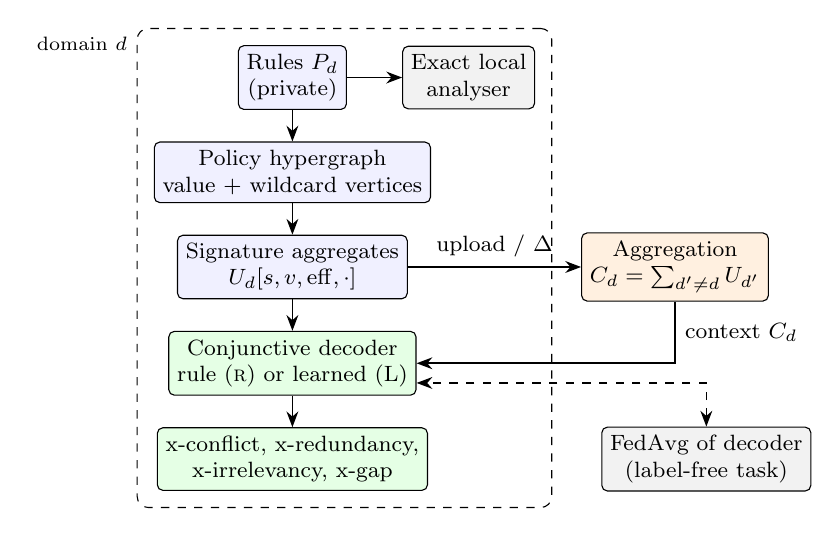
\begin{tikzpicture}[font=\footnotesize, node distance=4mm and 7mm,
  box/.style={draw, rounded corners=2pt, align=center, inner sep=3pt, fill=#1},
  box/.default={white}, arr/.style={-{Stealth[length=2mm]}, semithick}]
\node[box=blue!6] (pol) {Rules $P_d$\\(private)};
\node[box=gray!10, right=of pol] (loc) {Exact local\\analyser};
\node[box=blue!6, below=of pol] (hg) {Policy hypergraph\\value + wildcard vertices};
\node[box=blue!6, below=of hg] (agg) {Signature aggregates\\$U_d[s,v,\eff,\cdot]$};
\node[box=orange!12, right=22mm of agg] (srv) {Aggregation\\$C_d=\sum_{d'\neq d}U_{d'}$};
\node[box=green!10, below=of agg] (dec) {Conjunctive decoder\\rule (\R) or learned (L)};
\node[box=green!10, below=of dec] (out) {x-conflict, x-redundancy,\\x-irrelevancy, x-gap};
\node[box=gray!10, right=22mm of out] (fed) {FedAvg of decoder\\(label-free task)};
\draw[arr] (pol) -- (loc); \draw[arr] (pol) -- (hg); \draw[arr] (hg) -- (agg);
\draw[arr] (agg) -- node[above]{upload / $\Delta$} (srv);
\draw[arr] (srv.south) |- node[pos=.25, right]{context $C_d$} (dec.east);
\draw[arr] (agg) -- (dec); \draw[arr] (dec) -- (out);
\draw[arr, dashed, {Stealth[length=2mm]}-{Stealth[length=2mm]}] (fed.north) |- ($(dec.east)+(0,-2.5mm)$);
\node[draw, dashed, rounded corners, fit=(pol)(loc)(hg)(agg)(dec)(out), inner sep=6pt, label={[font=\scriptsize]above left:domain $d$}] {};
\end{tikzpicture}
\caption{Overview of \name for one domain. Solid arrows: data flow; dashed: optional federated training of the learned decoder. Only aggregates and decoder weights leave the domain.}
\label{fig:arch}
\end{figure}

\subsection{Hyperedge signatures and vertex aggregates}
\label{sec:agg}
Let $h$ be a hash function, salted with a key shared by the members of a scope, that maps a rule identifier to one of $B$ bins, and let $\sigma(r)\in\{0,1\}^B$ be the one-hot \emph{signature} of bin $h(r)$. Domain $d$ computes, for every scope $s$ it belongs to, every vertex $u\in\mathcal{V}$ and each effect $c$,
\begin{equation}
U_d[s,u,c]=\sum_{r\in P_d:\ \scp(r)=s,\ \eff(r)=c,\ u\in e(r)}\sigma(r)\ \in\mathbb{N}^B .
\label{eq:agg}
\end{equation}
Entry $b$ counts the rules of $d$ in scope $s$ with effect $c$ that are incident to $u$ and hash to bin $b$. For entity vertices, $d$ also publishes $L_d[v]=\mathrm{alive}(v)$ for the entities it owns. The aggregate has at most $\sum_r |e(r)|$ non-zero entries, independent of $B$. Each member receives the \emph{context}
\begin{equation}
C_d=\sum_{d'\neq d}U_{d'}+\xi,\qquad \Lambda_d=\sum_{d'\neq d}L_{d'}+\xi',
\label{eq:ctx}
\end{equation}
where $\xi,\xi'$ are optional zero-mean Gaussian noise terms of standard deviation $\sigma_{\!n}$ (Section~\ref{sec:privacy}). With secure aggregation~\cite{bonawitz2017practical} the server learns only the sums.

\subsection{Conjunctive decoding}
\label{sec:decode}
For a hyperedge $e$ of domain $d$ with scope $s$ and an effect channel $c$, define per attribute $a$ the \emph{overlap evidence} and the \emph{subsumption evidence}, both vectors in $\mathbb{R}^B$:
\begin{align}
\mathrm{ov}_a(e,c)&=C_d[s,(a,\ast),c]+
\begin{cases}\sum_{v\in D_a}C_d[s,(a,v),c] & \text{if } e_a=\ast,\\[2pt]
\sum_{v\in e_a}C_d[s,(a,v),c] & \text{otherwise,}\end{cases}\label{eq:ov}\\
\mathrm{sub}_a(e,c)&=C_d[s,(a,\ast),c]+
\begin{cases}0 & \text{if } e_a=\ast,\\[2pt]
\min_{v\in e_a}C_d[s,(a,v),c] & \text{otherwise.}\end{cases}\label{eq:sub}
\end{align}
Eq.~\eqref{eq:ov} mirrors the overlap condition: a foreign rule is compatible with $e$ on $a$ if it is a wildcard on $a$, or $e$ is, or they share a value. Eq.~\eqref{eq:sub} mirrors subsumption: the foreign rule is a wildcard on $a$, or contains every value of $e$. Evidence is then combined \emph{conjunctively} across attributes, bin by bin:
\begin{equation}
\mathrm{OV}(e,c)=\min_{a\in\mathcal{A}}\mathrm{ov}_a(e,c),\qquad \mathrm{SUB}(e,c)=\min_{a\in\mathcal{A}}\mathrm{sub}_a(e,c).
\label{eq:conj}
\end{equation}
A bin of $\mathrm{OV}$ is positive only if, on \emph{every} attribute, some foreign rule of that bin is compatible with $e$.

\paragraph{Rule decoder (\name-\R)} With $\bar c$ the effect opposite to $\eff(e)$ and threshold $\tau=\tfrac12$:
\begin{align*}
\text{x-conflict}(e)&\iff \max_b \mathrm{OV}(e,\bar c)_b>\tau,\\
\text{x-redundancy}(e)&\iff \max_b \mathrm{SUB}(e,\eff(e))_b>\tau,\\
\text{x-gap}(q)&\iff \max_b \textstyle\sum_c\mathrm{OV}(q,c)_b\le\tau,\\
\text{x-irrelevancy}(e)&\iff \exists a:\ \max_{v\in e_a}\big(L_d[v]+\Lambda_d[v]\big)\le\tau,
\end{align*}
where the last test ranges over constrained entity attributes with at least one foreign-owned value.

\subsection{Guarantees}
\begin{proposition}[One-sided error]
\label{prop:sound}
With $\sigma_{\!n}=0$ and any $B\ge1$, \name-\R{} flags every x-conflict and every x-redundancy, decides x-irrelevancy exactly, and every request it flags as an x-gap is one.
\end{proposition}
\begin{proof}
Let $r'\in F(e)$ overlap $e$ with the opposite effect and let $b=h(r')$. Fix an attribute $a$. If $r'_a=\ast$, $r'$ is incident to $(a,\ast)$ and contributes $1$ to $C_d[s,(a,\ast),\bar c]_b$. Otherwise $r'$ is incident to its value vertices in $D_a$; if $e_a=\ast$ these are all summed in \eqref{eq:ov}, and if $e_a\neq\ast$ overlap gives a shared $v\in e_a\cap r'_a$ whose term is summed. In every case $\mathrm{ov}_a(e,\bar c)_b\ge1$, so $\mathrm{OV}(e,\bar c)_b\ge1>\tau$. For redundancy let $e\sqsubseteq r'$ with equal effect. If $r'_a=\ast$ the wildcard term is $\ge1$; otherwise $e_a\neq\ast$ and $e_a\subseteq r'_a$, so every $v\in e_a$ has $C_d[s,(a,v),c]_b\ge1$ and so has the minimum in \eqref{eq:sub}. Hence $\mathrm{SUB}(e,c)_b\ge1$. If a foreign rule matches request $q$, the same argument with $e_a=\{q_a\}$ gives a bin with $\sum_c\mathrm{OV}(q,c)_b\ge1$, so $q$ is not flagged; contrapositively a flagged gap is a true gap. Liveness sums are exact without noise.
\end{proof}

\begin{proposition}[False-positive bound]
\label{prop:fp}
Model $h$ as uniform and independent over rules. Let $e$ have no x-conflict and let $N$ be the number of opposite-effect rules in $F(e)$. With $\sigma_{\!n}=0$, \name-\R{} flags $e$ with probability at most $N(N-1)/(2B)$. The same bound holds for x-redundancy with $N$ the number of same-effect foreign rules, and for the probability that a true x-gap is missed with $N=|F(q)|$.
\end{proposition}
\begin{proof}
A flag requires a bin $b$ with $\mathrm{ov}_a(e,\bar c)_b\ge1$ for all $a$, i.e.\ for each attribute some opposite-effect foreign rule in bin $b$ compatible with $e$ on that attribute. No single rule is compatible on all attributes, since it would overlap $e$. So at least two distinct rules among the $N$ share bin $b$. Two given rules collide with probability $1/B$; a union bound over the $\binom N2$ pairs gives the claim. The other cases are identical.
\end{proof}
The bound is loose, because it ignores that the colliding rules must jointly cover all attributes, but it identifies the governing ratio: errors vanish as $B$ grows relative to $N^2$ and appear only as extra conflicts and redundancies or hidden gaps. An auditor can therefore treat a negative answer for conflict and redundancy as definitive.

\subsection{Dynamics: exact delta maintenance}
\label{sec:delta}
\begin{proposition}[Delta exactness]
\label{prop:delta}
Let $P_d$ change to $P'_d$ by removing a set $R^-$ and inserting a set $R^+$ of rules. Then $U'_d=U_d+U(R^+)-U(R^-)$, where $U(\cdot)$ applies \eqref{eq:agg} to the given rules only; the number of non-zero entries of the delta is at most $\sum_{r\in R^+\cup R^-}|e(r)|$.
\end{proposition}
\begin{proof}
Eq.~\eqref{eq:agg} is a sum over rules of terms that depend on one rule each.
\end{proof}
A rule modification is a removal followed by an insertion; an entity that joins or leaves changes one entry of $L_d$. A domain therefore uploads a sparse delta proportional to the number of changed rules, the server adds it to the running sum, and members refresh only the affected context entries. No retraining is involved, because the rule decoder has no parameters and the learned decoder (below) depends on the context only through statistics whose distribution does not change with a single update. Algorithm~\ref{alg:dyfhl} summarises the protocol.

\begin{algorithm}[t]
\caption{\name at domain $d$ (server steps marked \textsc{srv})}
\label{alg:dyfhl}
\begin{algorithmic}[1]
\State run the exact local analyser on $P_d$ \Comment{intra-domain anomalies}
\State build $U_d$, $L_d$ by \eqref{eq:agg}; upload \Comment{initial exchange}
\State \textsc{srv}: $T\gets\sum_{d}U_d$; send $C_d=T-U_d\,(+\xi)$ to each member
\Loop\ on a policy or entity event $(R^-,R^+)$ at $d$
  \State re-run the local analyser on the affected rules
  \State $\Delta\gets U(R^+)-U(R^-)$; $U_d\gets U_d+\Delta$; upload $\Delta$ \Comment{Prop.~\ref{prop:delta}}
  \State \textsc{srv}: $T\gets T+\Delta$; forward $\Delta$ to the other members of the touched scopes
\EndLoop
\ForAll{own hyperedge or request $e$ whose context changed}
  \State compute $\mathrm{OV}(e,\cdot)$, $\mathrm{SUB}(e,\cdot)$ by \eqref{eq:ov}--\eqref{eq:conj}
  \State decode with the rule (\R) or the learned heads (L)
\EndFor
\end{algorithmic}
\end{algorithm}

\subsection{Learned decoder and label-free federated training}
\label{sec:learn}
With noise, or with a small $B$, a fixed threshold on $\max_b$ is not obviously the best decision. \name-L replaces it by four small networks, one per task. Each receives permutation-invariant statistics of the relevant evidence vector(s) over bins (the three largest entries, the mean, the standard deviation, and the fractions of bins above $0.3$, $0.5$ and $0.8$) for $\mathrm{OV}$, $\mathrm{SUB}$ and the attribute-mean of $\mathrm{ov}_a$; the irrelevancy head receives the liveness evidence. Each head is a two-hidden-layer perceptron (32 and 16 units).

No cross-domain labels exist to train on, since producing them is the problem. We use a \emph{pseudo-domain} task that every domain can build alone. At each local step, domain $d$ (i) splits its rules at random into two halves, (ii) adds synthetic variants of its own rules (copies with flipped or kept effect, generalised by dropping an attribute or specialised by constraining a wildcard, placed in the opposite half; some refer to entities $d$ owns, with random liveness), (iii) computes with its exact local analyser the labels of Definition~\ref{def:anom} with the other half playing the foreign domain, and (iv) decodes each half from the aggregate of the other, to which noise of the deployment level is added. The heads are trained with binary cross-entropy on these labels and averaged across domains with FedAvg~\cite{mcmahan2017communication}. Only the weights of the heads are shared. An optional \emph{learned message channel} lets each rule add a trained embedding of its vertex set to its signature; it is evaluated as an ablation.

\subsection{Complexity and communication}
Building $U_d$ costs $O(\sum_{r\in P_d}|e(r)|)$. Decoding one hyperedge costs $O(A\,B)$ after $O(A)$ gathers, so a domain with $n_d$ shared-scope rules spends $O(n_d A B)$, against $O(n^2A)$ for the pooled oracle on $n=\sum_d n_d$ rules. The initial upload has at most $\sum_r|e(r)|\le n_d(A+\sum_a(|r_a|-1))$ non-zeros; a delta has that many per changed rule. The receiver's context is dense in the worst case, $|M_s|$-independent, of size $S_d(|\mathcal V|)\,2B$ for $S_d$ scopes.

\subsection{Privacy analysis}
\label{sec:privacy}
\paragraph{What is exchanged} A member receives, per scope, vertex, effect and bin, the number of foreign rules incident to that vertex. It never receives a rule, an identifier, or which domain a count comes from when the scope has more than two members.

\paragraph{What can be inferred} The bin index links the vertices of a rule. If a bin of the context holds a single foreign rule, its non-zero entries across vertices are exactly that rule's hyperedge, and the rule is revealed. The expected number of foreign rules per bin is $N_s/B$ for $N_s$ foreign rules in scope $s$, so $B$ controls a direct trade-off: Proposition~\ref{prop:fp} wants $B\gg N^2$, while hiding rules among others wants $B\ll N_s$. In a two-member scope the context equals the peer's aggregate. \name therefore achieves \emph{data minimisation}: domains disclose which attribute values their shared-scope rules use, mixed within bins, instead of the rules, and disclose nothing about rules outside shared scopes. It does not achieve secrecy of shared-scope rules against a determined member when $B$ is large.

\paragraph{Noise and differential privacy} Adding or removing one rule changes at most $2A$ entries of \eqref{eq:agg} by one when value sets have at most two values, an $\ell_2$ sensitivity of $\sqrt{2A}$. The Gaussian mechanism~\cite{dwork2014algorithmic} then gives $(\varepsilon,\delta)$-differential privacy at rule level per release for $\sigma_{\!n}=\sqrt{2A}\sqrt{2\ln(1.25/\delta)}/\varepsilon$. Section~\ref{sec:noise} shows that the accuracy of the conjunctive decoder collapses well before $\sigma_{\!n}$ reaches the values that small $\varepsilon$ requires, because a minimum over attributes amplifies noise. We regard this as a property of any decoder that must certify a conjunction from independent noisy counts.

%% ============================================================================
\section{Experimental setup}
\label{sec:setup}

\paragraph{Research questions} RQ1: how close does \name come to the pooled oracle, and how do alternatives that do not pool policies compare? RQ2: which design elements matter? RQ3: how do sketch size and noise trade accuracy against communication and privacy? RQ4: how does the approach scale with rules and domains? RQ5: what does delta maintenance buy under churn?

\paragraph{Datasets} No public corpus of multi-domain policies with cross-domain anomaly labels exists. We build three benchmarks from three rule sources with one procedure, and state plainly what is real and what is generated.
\begin{itemize}
\item \emph{Agentic} (synthetic). Eight attributes: subject type (agent, MCP server, tool, application, legacy system, human), role, clearance, resource type, sensitivity, action, trust context and tool identity (60 entities). Each domain has its own Dirichlet preference over values, so domains are non-IID.
\item \emph{XS-ABAC} (derived). Attribute data of the healthcare, university, project-management and online-video case studies of Xu and Stoller~\cite{xu2015mining}: real users and resources with their attribute values. Rules are generated as conjunctions of attribute-value conditions taken from real user and resource records of one case study; the original ten or so rules per case study are too few to form a benchmark.
\item \emph{AMZ-Access} (derived). The Amazon employee access data~\cite{amazon2013access}: each rule keeps the resource and three to five role attributes of a real access record (restricted to the 25 most frequent values per column).
\end{itemize}
For each source we create $K=6$ domains and six collaboration scopes with two to four members, 400 shared-scope rules per domain, and 250 candidate requests per domain of which those not covered locally are kept. To control prevalence, 10\% of the rules are replaced by an overlapping variant of a foreign rule with the opposite effect, 10\% by a variant subsumed by a foreign rule, and 8\% refer to decommissioned foreign entities (15\% of entities are dead). \emph{All labels are computed by the pooled exact oracle on the final rule sets}, so naturally occurring anomalies are labelled as well; injection only shifts prevalence. Table~\ref{tab:data} gives the resulting statistics. The domain and scope structure of the two derived benchmarks is imposed by us; only the attribute data are real.

\begin{table}[t]
\caption{Benchmark statistics (means over seeds). Prevalence is the fraction of positive labels per task.}
\label{tab:data}
\centering\footnotesize
\resizebox{\linewidth}{!}{%
\begin{tabular}{lrrrrrrr}
\toprule
& & & & \multicolumn{4}{c}{Prevalence (\%)}\\ \cmidrule(l){5-8}
Benchmark & $A$ & Rules & Requests & x-conflict & x-redund. & x-irrelev. & x-gap\\
\midrule
Agentic & 8 & \nagenticrules & \nagenticreq & \prevagenticcon & \prevagenticred & \prevagenticirr & \prevagenticgap\\
XS-ABAC & 15 & \nxustollerrules & \nxustollerreq & \prevxustollercon & \prevxustollerred & \prevxustollerirr & \prevxustollergap\\
AMZ-Access & 11 & \namazonrules & \namazonreq & \prevamazoncon & \prevamazonred & \prevamazonirr & \prevamazongap\\
\bottomrule
\end{tabular}}
\end{table}

\paragraph{Methods compared} None of the following pools policies, except where noted.
\begin{itemize}
\item \emph{RF, local features}: a random forest on each hyperedge's own incidence row, trained on 20\% of the oracle labels and tested on the rest. It receives audited labels that \name does not need.
\item \emph{RF + count context}: the same with per-vertex foreign rule counts as additional features.
\item \emph{Local-only}: the learned decoder without any exchange.
\item \emph{FedHGNN (count completion)}: our re-implementation of the idea of FedHGL~\cite{luo2024fedhgl} in this setting: domains exchange per-vertex counts and learned embeddings without scope partition, pooled over the hyperedge's vertices (mean, max, min), trained with FedAvg on the same label-free task. It is not the authors' code.
\item \emph{FedGCN (clique expansion)}: the same, followed by a graph convolution over the local clique expansion of the hypergraph.
\item \emph{\name-L} and \emph{\name-\R}: learned and rule decoder, $B=512$, $\sigma_{\!n}=0$.
\end{itemize}
The pooled oracle scores 1 on every metric by definition and is the reference, not a competitor.

\paragraph{Metrics and protocol} Per task we report F1 of the positive class at threshold $0.5$ and the area under the precision--recall curve (AUPRC); macro averages are over the four tasks. Main results use five seeds (data generation and training), other studies three; we report mean and sample standard deviation and paired $t$-tests on seeds. Federated training uses 20 rounds of 5 local Adam steps (learning rate $10^{-2}$, 256 hyperedges per step). Experiments ran on two CPU cores without a GPU. The value-set size per attribute is at most two in all benchmarks.

\paragraph{Reproducibility} The code, the experiment runner, the figure generator that produces every number in this paper from the result files, a Colab notebook and a Streamlit explorer with hypergraph projections of the anomalies are in the accompanying repository.

%% ============================================================================
\section{Results}
\label{sec:results}

\subsection{RQ1: comparison with non-pooling alternatives}
Table~\ref{tab:main} reports the main comparison at $B=512$. \name-\R{} obtains macro-F1 of \mainagenticR{} (Agentic), \mainxustollerR{} (XS-ABAC) and \mainamazonR{} (AMZ-Access). The strongest baseline in macro-F1 is on every benchmark a random forest trained on audited labels (\mainagenticbest, \mainxustollerbest{} and \mainamazonbest). The paired difference to \name-\R{} is $\mainagenticgain$ on Agentic ($p=\mainagenticp$) and $\mainamazongain$ on AMZ-Access ($p=\mainamazonp$). On XS-ABAC it is $\mainxustollergain$ ($p=\mainxustollerp$): at this sketch size \name-\R{} is on par with, not better than, a supervised model that was given 20\% of the oracle's labels.

The XS-ABAC deficit is confined to x-gap (F1 \mainxustollerRgap). This benchmark has the densest overlap structure (x-conflict prevalence \prevxustollercon\%), so many foreign rules are partially compatible with each request, bins fill up, and collisions hide true gaps: recall of x-gap is \mainxustollerRgaprec{} at precision \mainxustollerRgapprec. The error disappears with a larger sketch; at $B=4096$ the rule decoder reaches macro-F1 \skxustollerruleBmmmmxcvi{} on XS-ABAC (Section~\ref{sec:sketch}).

Three further observations explain the table. First, x-irrelevancy needs one number per entity and is decided exactly by the rule decoder; the baselines that receive liveness counts come close, those that do not fail. The learned decoder is unreliable on this task outside Agentic (F1 \mainxustollerLirr{} on XS-ABAC, \mainamazonLirr{} on AMZ-Access): there a domain owns only a handful of entities, so its pseudo-domain task contains almost no positive example. Second, for x-conflict and x-redundancy the federated baselines often score an F1 of zero while their AUPRC is not negligible: per-vertex counts say that foreign rules use the same values, not that one foreign rule is compatible on all attributes, so scores are weakly informative and rarely cross the decision threshold. Supplying audited labels does not repair this on Agentic and AMZ-Access; on XS-ABAC, where \prevxustollercon\% of the rules are in conflict, predicting the majority class already gives a high F1. Third, \name-L and \name-\R{} are indistinguishable on x-conflict, the rule decoder is clearly better on x-redundancy on Agentic and AMZ-Access, and the learned decoder is better on x-redundancy and x-gap on XS-ABAC, where the fixed threshold suffers most from collisions. In macro-F1 the rule decoder is ahead on all three benchmarks (paired $p=\mainagenticpRL$, $\mainxustollerpRL$ and $\mainamazonpRL$). In ranking quality the order reverses: \name-L has the highest macro-AUPRC of all methods on every benchmark (\mainagenticLap, \mainxustollerLap{} and \mainamazonLap, against \mainagenticRap, \mainxustollerRap{} and \mainamazonRap{} for the rule decoder, whose outputs are binary). The learned decoder is therefore useful for prioritising findings and for small sketches, and the rule decoder for decisions.

Relative to the oracle, the error of \name-\R{} is one-sided, as Proposition~\ref{prop:sound} states: recall for x-conflict and x-redundancy is \mainagenticRconrec{} and \mainagenticRredrec{} on Agentic, \mainxustollerRconrec{} and \mainxustollerRredrec{} on XS-ABAC, \mainamazonRconrec{} and \mainamazonRredrec{} on AMZ-Access, with precision between \mainxustollerRredprec{} and \mainamazonRconprec; precision for x-gap is \mainagenticRgapprec{} on all three. Section~\ref{sec:sketch} shows that the residual error is a function of $B$.

\begin{table}[t]
\caption{Cross-domain anomaly detection without pooling policies: F1 per task, macro-F1 and macro-AUPRC (mean $\pm$ std over seeds). Best mean per column and benchmark in bold. $^\dagger$Trained on 20\% of the oracle labels, tested on the remaining 80\%.}
\label{tab:main}
\centering\scriptsize
\setlength{\tabcolsep}{3pt}
\resizebox{\linewidth}{!}{%
\begin{tabular}{lcccccc}
\toprule
Method & x-conflict & x-redund. & x-irrelev. & x-gap & macro-F1 & macro-AUPRC\\
\midrule
\rawinput{generated/tab_main}
\bottomrule
\end{tabular}}
\end{table}

\subsection{RQ2: ablations}
\label{sec:ablation}
\paragraph{Structure} Table~\ref{tab:abl_s} removes one structural element at a time from \name-\R. Every element matters. Without scope partition, rules of unrelated scopes fill the same bins and the decoder flags almost everything. Without conjunctive pooling the evidence is pooled over the hyperedge's vertices regardless of attribute, which loses the semantics of overlap. Without wildcard vertices, foreign rules that leave an attribute unconstrained are invisible on that attribute and the conjunction fails for most true anomalies. Replacing the signature sketch by plain counts ($B=1$) keeps the structure but removes the ability to tell one compatible rule from several partially compatible ones.

\begin{table}[t]
\caption{Structural ablation of \name-\R{} ($B=512$): macro-F1 per benchmark (mean $\pm$ std, three seeds) and F1 per task averaged over benchmarks.}
\label{tab:abl_s}
\centering\scriptsize
\setlength{\tabcolsep}{3pt}
\resizebox{\linewidth}{!}{%
\begin{tabular}{lccccccc}
\toprule
& \multicolumn{3}{c}{macro-F1} & \multicolumn{4}{c}{F1 per task (mean over benchmarks)}\\ \cmidrule(lr){2-4}\cmidrule(l){5-8}
Variant & Agentic & XS-ABAC & AMZ-Access & x-conf. & x-red. & x-irr. & x-gap\\
\midrule
\rawinput{generated/tab_abl_structure}
\bottomrule
\end{tabular}}
\end{table}

\paragraph{Learning} Table~\ref{tab:abl_l} varies the training of \name-L. The synthetic variants are the one indispensable ingredient: without them a domain's two halves contain too few subsumption pairs and x-redundancy is not learned (F1 \ablleapseudoanomalyared). Federated averaging helps on Agentic (\ablleafulllearneddecagentic{} against \ablleaFedAvglocaltraagentic{} for purely local training) and makes no difference on AMZ-Access. The learned message channel leaves the result unchanged on both benchmarks. Letting the heads see the hyperedge's own features (``priors'') lowers macro-F1 on Agentic and raises it on AMZ-Access, where it stabilises the irrelevancy head. Adding recombined rules so that the pseudo-foreign side is as dense as a real context hurts on Agentic. No variant reaches the rule decoder of Table~\ref{tab:abl_s}, and the standard deviations are several times larger than the rule decoder's. We read the two tables together as evidence that the structure of the aggregation, not the learning, carries the method.

\begin{table}[t]
\caption{Learning ablation of \name-L ($B=512$): macro-F1 per benchmark (mean $\pm$ std, three seeds) and F1 per task averaged over the two benchmarks.}
\label{tab:abl_l}
\centering\scriptsize
\setlength{\tabcolsep}{3pt}
\resizebox{\linewidth}{!}{%
\begin{tabular}{lcccccc}
\toprule
& \multicolumn{2}{c}{macro-F1} & \multicolumn{4}{c}{F1 per task}\\ \cmidrule(lr){2-3}\cmidrule(l){4-7}
Variant & Agentic & AMZ-Access & x-conf. & x-red. & x-irr. & x-gap\\
\midrule
\rawinput{generated/tab_abl_learning}
\bottomrule
\end{tabular}}
\end{table}

\subsection{RQ3: sketch size, communication and noise}
\label{sec:sketch}
\paragraph{Sketch size} Fig.~\ref{fig:sketch} varies $B$. For \name-\R{} macro-F1 rises monotonically with $B$, from \skagenticruleBlxiv{} at $B=64$ to \skagenticruleBdxii{} at $B=512$ and \skagenticruleBmmmmxcvi{} at $B=4096$ on Agentic (\skamazonruleBlxiv, \skamazonruleBdxii{} and \skamazonruleBmmmmxcvi{} on AMZ-Access; \skxustollerruleBlxiv, \skxustollerruleBdxii{} and \skxustollerruleBmmmmxcvi{} on XS-ABAC), as Proposition~\ref{prop:fp} predicts: with enough bins the decoder reproduces the pooled oracle. The number of non-zeros a domain uploads does not depend on $B$ (\skagenticbytesBdxii~kB on Agentic at four bytes per value); only the dense context held by the receiver grows. On Agentic the learned decoder is slightly better than the rule up to $B=256$, where the fixed threshold fires on most hyperedges while the heads can still use the bin statistics; from $B=512$ upward, and on AMZ-Access at every $B$, the rule decoder is better.

\begin{figure}[t]
\centering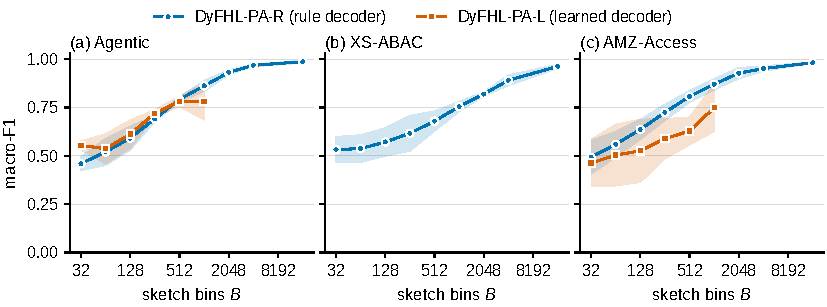
\includegraphics[width=\linewidth]{generated/fig_sketch}
\caption{Effect of the number of sketch bins $B$ on macro-F1 (left, centre; mean $\pm$ std over three seeds) and on the size of one domain's upload (right; non-zero entries versus dense tensor).}
\label{fig:sketch}
\end{figure}

\paragraph{Noise}
\label{sec:noise}
Fig.~\ref{fig:noise} and Table~\ref{tab:noise} add Gaussian noise of standard deviation $\sigma_{\!n}$ to every context entry. Accuracy holds up to $\sigma_{\!n}\approx0.1$ and then falls: on Agentic \name-\R{} goes from \nzagenticRsApA{} without noise to \nzagenticRsApB{} at $0.1$, \nzagenticRsApD{} at $0.3$ and \nzagenticRsApF{} at $0.5$; on AMZ-Access from \nzamazonRsApA{} to \nzamazonRsApB, \nzamazonRsApD{} and \nzamazonRsApF. Training the learned decoder with the deployment noise does not make it more robust: it is below the rule decoder at every noise level on both benchmarks. The table translates $\sigma_{\!n}$ into the per-release $\varepsilon$ of the Gaussian mechanism at $\delta=10^{-5}$. The noise levels at which the method works correspond to $\varepsilon$ in the hundreds, which is not a meaningful guarantee; $\varepsilon<10$ would need $\sigma_{\!n}$ of about 2, far beyond the point where the conjunction is destroyed.

\begin{figure}[t]
\centering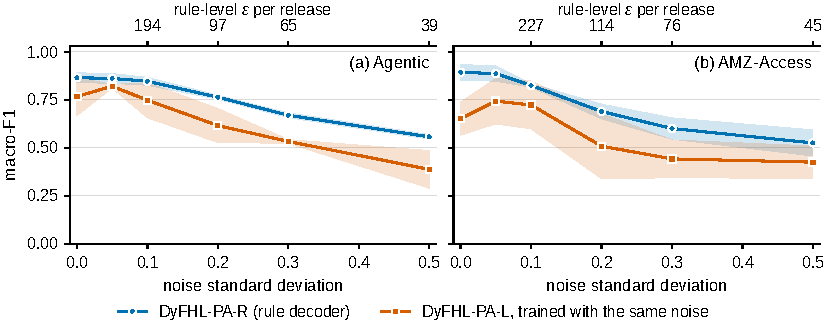
\includegraphics[width=.8\linewidth]{generated/fig_noise}
\caption{Macro-F1 under additive Gaussian noise on the context (mean $\pm$ std over three seeds).}
\label{fig:noise}
\end{figure}

\begin{table}[t]
\caption{Macro-F1 under context noise $\sigma_{\!n}$ and the corresponding rule-level $\varepsilon$ per release ($\delta=10^{-5}$, sensitivity $\sqrt{2A}$).}
\label{tab:noise}
\centering\scriptsize
\setlength{\tabcolsep}{3pt}
\begin{tabular}{lcccccc}
\toprule
& \multicolumn{3}{c}{Agentic} & \multicolumn{3}{c}{AMZ-Access}\\ \cmidrule(lr){2-4}\cmidrule(l){5-7}
$\sigma_{\!n}$ & $\varepsilon$ & \name-\R & \name-L & $\varepsilon$ & \name-\R & \name-L\\
\midrule
\rawinput{generated/tab_noise}
\bottomrule
\end{tabular}
\end{table}

\subsection{RQ4: scalability}
Fig.~\ref{fig:scale} grows the Agentic benchmark from 600 to 9{,}600 shared-scope rules. With $B$ fixed at 512, macro-F1 decreases from \scfixedfgaa{} to \scfixedfjgaa{} as bins fill up; with $B$ proportional to the rules per domain ($B=4n_d$) it decreases only from \scscaledfgaa{} to \scscaledfjgaa, at the price of decoding time. We must also report that at these sizes the pooled oracle is not slow: vectorised, it labels 9{,}600 rules in \scfixedojgaa~s, against \scfixedtjgaa~s for \name-\R{} with $B=512$ and \scscaledtjgaa~s with $B=4n_d$ (all domains, sequentially, on one core). The case for \name is that it does not need the policies in one place, not that it is faster. Macro-F1 as a function of the number of domains (with as many scopes as domains and $B=512$) is \scKd, \scKg, \scKj{} and \scKbc{} for $K=3,6,9,12$, without a trend: what matters is the number of rules per scope, not the number of domains.

\begin{figure}[t]
\centering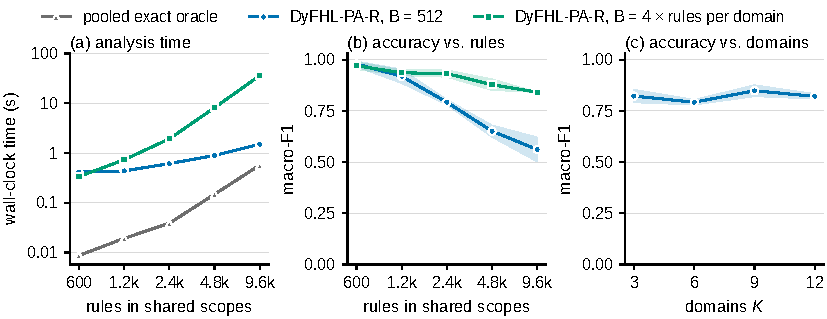
\includegraphics[width=\linewidth]{generated/fig_scale}
\caption{Scalability on Agentic. Left: wall-clock time of the pooled oracle and of \name-\R{} inference for all domains. Centre: macro-F1 versus number of rules for fixed and proportional $B$. Right: macro-F1 versus number of domains ($B=512$).}
\label{fig:scale}
\end{figure}

\subsection{RQ5: policy churn}
Fig.~\ref{fig:stream} replays ten steps in which 5\%, 10\% or 20\% of the rules are replaced and 5\% of the entities change liveness per step. The delta-maintained context is identical to a full recomputation at every step (largest absolute difference \stmaxerr), as Proposition~\ref{prop:delta} states, so \name-\R{} with deltas gives exactly the answers of a fresh exchange on the current policies. A context that is not refreshed degrades with the cumulative churn: after ten steps at 20\% churn macro-F1 on Agentic is \stagenticstaleApC{} against \stagenticdeltaApC{} with deltas (\stamazonstaleApC{} against \stamazondeltaApC{} on AMZ-Access). The delta-maintained curve is not flat either. This is a property of the generated stream, not of the maintenance: replaced rules are less often variants of current foreign rules, so the prevalence of x-conflict falls (from 28\% to 22\% at 20\% churn on Agentic) and, at a constant false-positive rate, so does F1. The delta upload is \stagenticratioApAF\%, \stagenticratioApB\% and \stagenticratioApC\% of a full upload at the three churn rates on Agentic (\stamazonratioApAF\%, \stamazonratioApB\%, \stamazonratioApC\% on AMZ-Access), twice the churn rate, since removals and insertions are both sent. At this scale computing a delta is not faster than recomputing the aggregate (\sttdelta~ms against \sttfull~ms per step for all domains); the saving is in communication.

\begin{figure}[t]
\centering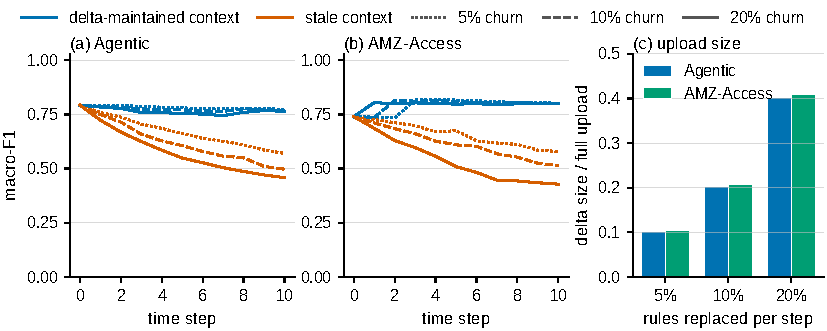
\includegraphics[width=\linewidth]{generated/fig_stream}
\caption{Policy stream. Left, centre: macro-F1 of \name-\R{} over time with a delta-maintained and a stale context. Right: size of the delta upload relative to a full upload.}
\label{fig:stream}
\end{figure}

%% ============================================================================
\section{Discussion and limitations}
\label{sec:discussion}

\paragraph{What the results support} Encoding the logic of rule overlap in the aggregation recovers most of the pooled analysis from additive, hashed vertex statistics, with errors on one known side, exact incremental updates, and communication proportional to the number of rules. Federated graph or hypergraph completion that shares per-vertex features without that logic does not.

\paragraph{Learning plays a secondary role} The name of the approach reflects its starting point: a federated hypergraph neural model. The experiments led elsewhere. The learned decoder ranks findings better than the rule and can help when the sketch is small or the overlap structure is dense, but it does not improve decisions overall, its variance across runs is high, and the learned message channel adds nothing. We kept both in the paper and the code because the comparison is informative, and because a learned component may pay off in settings we did not test: soft attribute matching (hierarchies, numeric ranges), where compatibility is not set intersection, is the most plausible.

\paragraph{Privacy} \name removes the need to hand policies to a third party and limits disclosure to shared scopes, but it is not a private protocol in the cryptographic or differential sense: large sketches expose the structure of individual foreign rules to scope members, and the noise needed for small $\varepsilon$ destroys the signal (Section~\ref{sec:noise}). Deployments should choose $B$ from the tolerable false-positive rate and the acceptable mixing $N_s/B$, use secure aggregation, and treat scope membership as a trust decision. Combining the hypergraph aggregation with multi-party computation of the per-bin minimum is the natural way to remove this leakage.

\paragraph{Validity} (i) The agentic benchmark is synthetic, and the domain structure of the derived benchmarks is imposed; no public multi-domain policy corpus exists to check against. (ii) Labels come from an oracle for the rule language of Section~\ref{sec:problem}: conjunctions of set-membership conditions, with at most two values per attribute in our data. Rule-combining algorithms, obligations, attribute hierarchies and relational constraints between subject and resource attributes (present in the original Xu--Stoller policies) are not modelled. (iii) The hash is assumed uniform; an adversarial member who knows the salt could craft collisions. (iv) The baselines are our re-implementations of ideas in a common framework, not the original systems. (v) Experiments are CPU-scale; the largest setting has 9{,}600 rules, a size at which the pooled oracle itself runs in under a second, so we make no claim about computational advantage. (vi) The learned decoder was trained for 100 local steps per domain; a longer schedule or a different architecture might change its ranking relative to the rule.

%% ============================================================================
\section{Conclusion}
\label{sec:conclusion}
We formulated cross-domain policy anomaly analysis as a problem on a policy hypergraph with wildcard vertices and showed that scope-partitioned vertex aggregates of hashed hyperedge signatures, decoded conjunctively across attributes, reproduce the pooled analysis with one-sided error bounded in $1/B$, without any domain reading another's rules, and with exact sparse updates under churn. On two of three benchmarks the approach is far ahead of every baseline at 512 bins, on the third it matches a supervised baseline that uses audited labels, and with 4096 bins it reproduces the oracle on all three; a fixed decoder is better than a federated, label-free learned one at decisions and worse at ranking; and additive noise is not a viable privacy mechanism for it. Future work will replace the plain exchange of bin counts by secure computation of the conjunction, extend the rule language to hierarchies and relational constraints where a learned compatibility function is needed, and evaluate on policies collected from deployed agent platforms.

\section*{CRediT authorship contribution statement}
\textbf{Mokhtar Sellami}: Conceptualization, Methodology, Software, Validation, Writing.

\section*{Declaration of competing interest}
The author declares no competing interests.

\section*{Declaration of generative AI in the writing process}
During the preparation of this work the author used an AI assistant (Claude, Anthropic) to help design and implement the experiments and to draft the manuscript. The author reviewed and edited the content and takes full responsibility for the publication.

\section*{Data availability}
Code and scripts that regenerate all results are in the accompanying repository. The Xu--Stoller case studies and the Amazon access data are public and are fetched by a script.

\bibliographystyle{elsarticle-num}
\bibliography{references}
\end{document}
